\chapter{Sparse Coding}
% Authors: Francesco Preta (Editor), Ambuj Ojha (Part1), Bingqian Deng (Part2)
% Lecture  date: 4/29/2019 part 1


%Beggining of Bingqian's part
\section{Energy-Based Unsupervised Learning}
Unsupervised learning can be approached through the optimization of an energy function. In order to do so, we need to model such function following a set of rules:
\begin{enumerate}
    \item Build the machine so that the volume of low energy stuff is constant;
    \item Push down of the energy of data points, push up everywhere else;
    \item Push down of the energy of data points, push up on chosen locations;
    \item Minimize the gradient and maximize the curvature around data points;
    \item Train a dynamical system so that the dynamics goes to the manifold;
    \item Use a regularizer that limits the volume of space that has low energy;
    \item If $E(Y) = ||Y - G(Y)||^2$, make $G(Y)$ as "constant" as possible;
    \item Adversarial training: generator tries to fool real/synthetic classifier.
\end{enumerate}% \begin{figure}[h!]
% \centering
% \includegraphics[width=1.0\linewidth]{19_ss_a.png}
% \caption{Daily productive hours: Feb.18 $\sim$ Apr.4 2019}
% \label{fig:dailyhour}
% \end{figure}


In particular, the main focus of the lecture will come from the sixth point, using sparse coding, sparse auto-encoders and Predictive Sparse Decomposition (PSD).

\subsection{The Decoder with Restricted Latent Variable Model}

In what follows, we will use the following notation: $Z$ is the latent variable, possibly high dimensional, $Y$ is the observed signal, $Y'$ is the prediction signal reconstructed through a decoder. Such reconstruction can be obtained by matrix multiplication or through a neural network in more sophisticated models. The mathematical formulation is as follows : 
\[Y'=\operatorname{Dec}(\mathbf{Z}) \quad \mathbf{Z}^{*}=\operatorname{argmin}\|Y-\operatorname{Dec}(\mathbf{Z})\|+R(\mathbf{Z})\]
When given the target, the goal is to find the latent $Z$ that minimizes the energy function. This has generally two terms, one is the residual error (the difference between the prediction and target) and the other is the regularizer on $Z$, which restricts the space in which we can find the optimum and increases regularity of the solutions. In sparse coding, the regularizer is usually the $L^1$ norm of $Z$, which has the effect of setting to zero most of the components. Fig. \ref{fig:decoder} shows the structure just described, while Fig.\ref{fig:energy} shows different types of energy functions.
\begin{figure}[H]
\centering
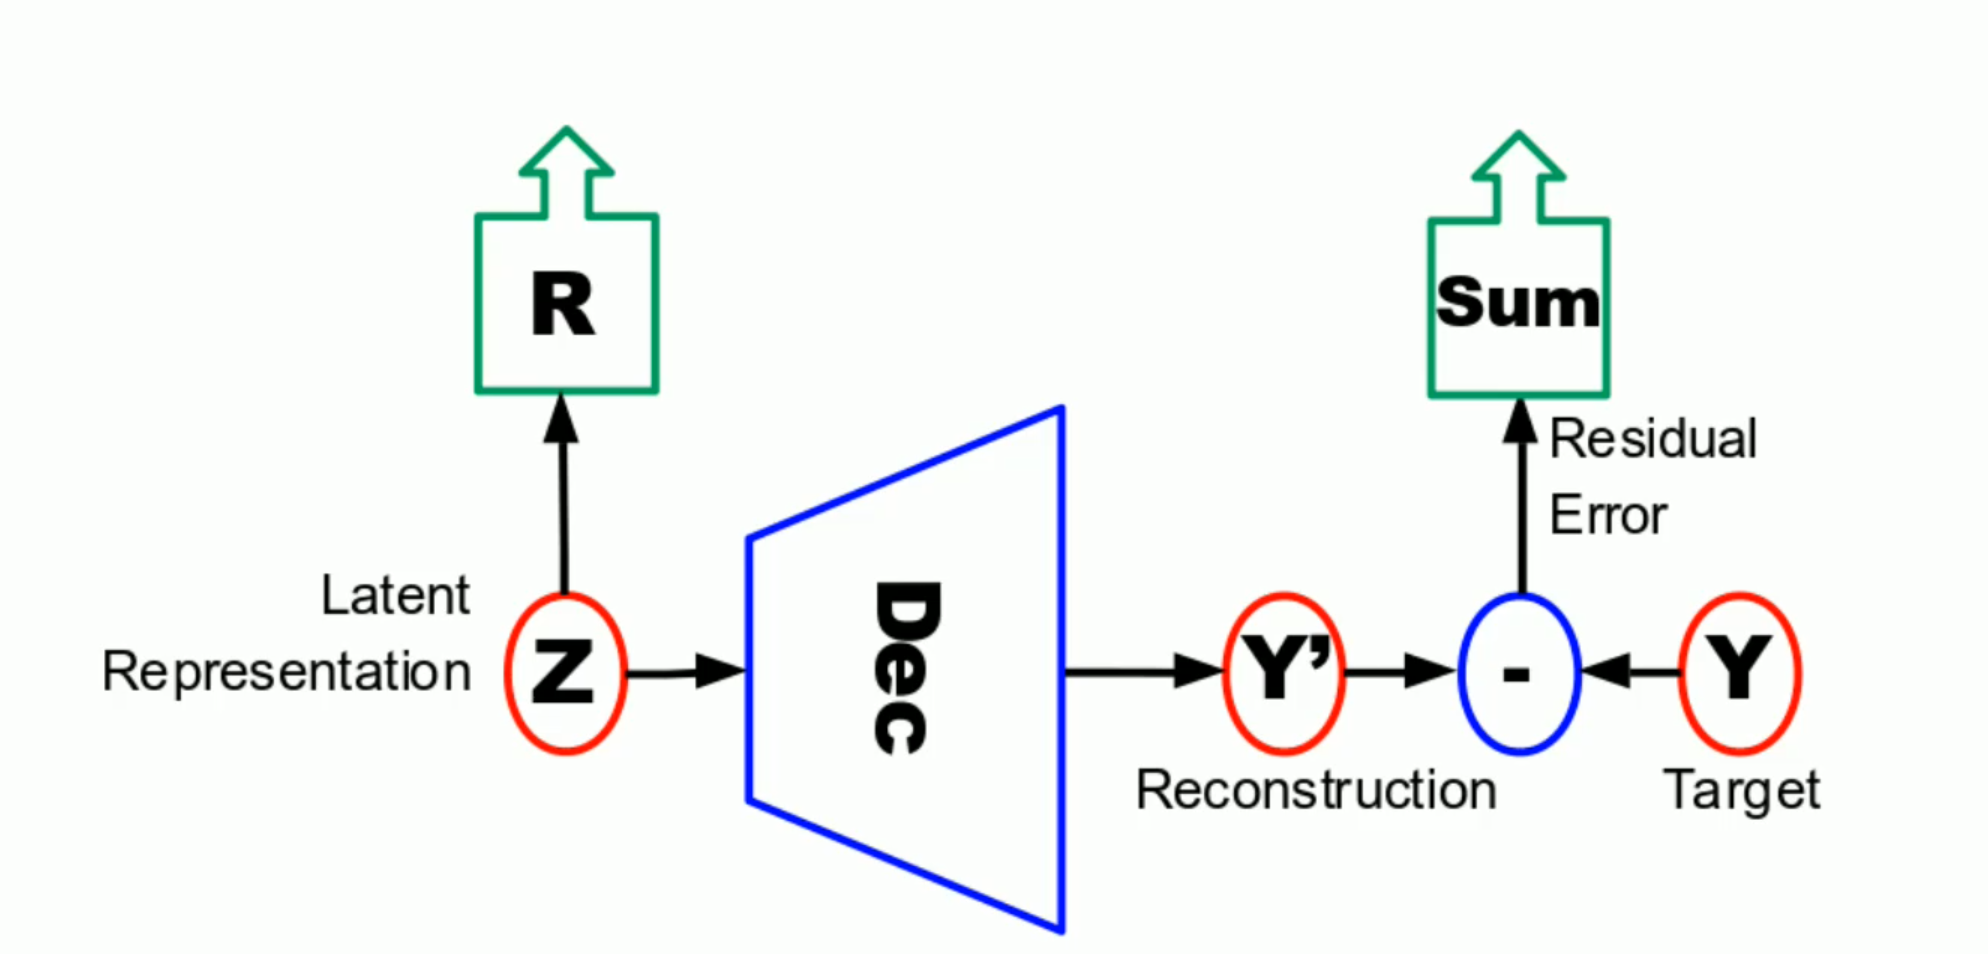
\includegraphics[width=1.0\linewidth]{lectures/12-a/decoder.png}
\caption{The Decoder with Restricted Latent Variable Model}
\label{fig:decoder}
\end{figure}
\begin{figure}[H]
\centering
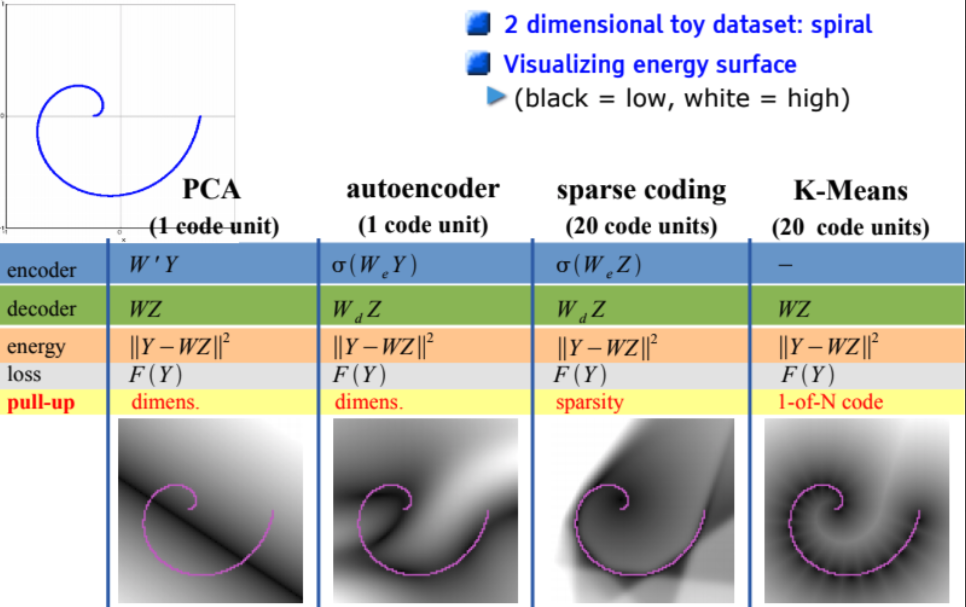
\includegraphics[width=0.8\linewidth]{lectures/12-a/ernergy.png}
\caption{Energy Functions of Various Methods}

\label{fig:energy}
\end{figure}
\section*{Sparse Coding and Sparse Modeling}

Fig \ref{fig:sparse} shows the scheme of sparse linear reconstruction \cite{olshausen1997sparse}, while fig \ref{fig:generative} shows the framework of performing inference in generative models.
The energy function is modeled as follows:
\[E\left(Y^{i}, Z\right)=\left\|Y^{i}-W_{d} Z\right\|^{2}+\lambda \sum_{j}\left|z_{j}\right|\]
\begin{figure}[H]
\centering
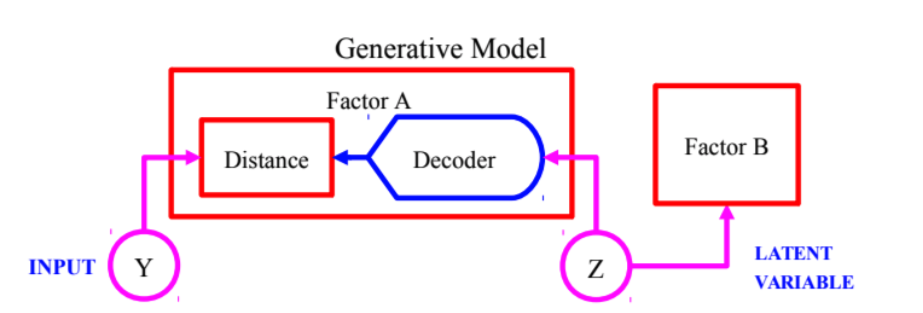
\includegraphics[width=1.0\linewidth]{lectures/12-a/generative.png}
\caption{Inference in a Generative Model}
\label{fig:generative}
\end{figure}

\begin{figure}[H]
\centering
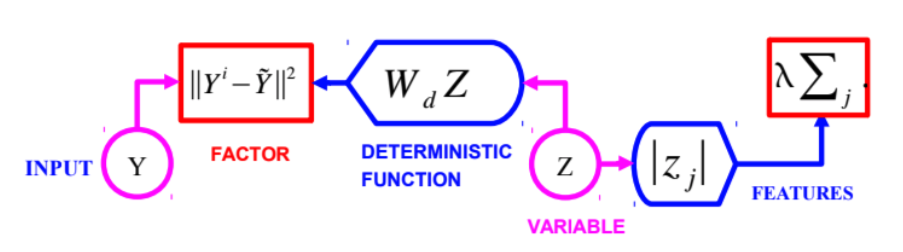
\includegraphics[width=1.0\linewidth]{lectures/12-a/sparse.png}
\caption{Sparse Coding}
\label{fig:sparse}
\end{figure}
$W_d$ is called the dictionary matrix, where the first term represents the reconstruction error and the second term deals with the sparsity. However, the optimization algorithm to find $Z$ for a fixed $Y$ is computationally expensive. The algorithm that deals with auto-encoding and the regularizer term is called ISTA (Iterative Shrinkage Threshold Algorithm). 

Fig \ref{encoder} shows the encoder architecture. Most ICA models and Product of Experts are examples of this architecture.

\begin{figure}[H]
\centering
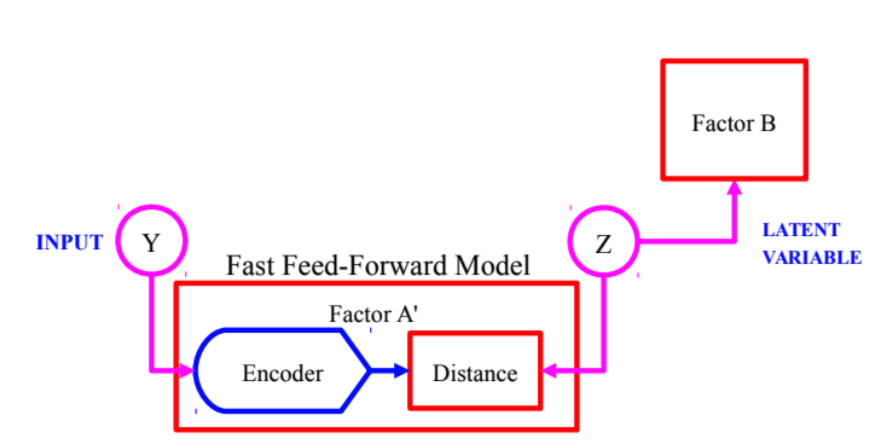
\includegraphics[width=1.0\linewidth]{lectures/12-a/encoder.png}
\caption{Encoder Architecture}
\label{encoder}
\end{figure}
Fig \ref{enco_deco} shows the encoder-decoder architecture. The input $Y$  is passed through a feed-forward model, possibly with a regularizer, to make a prediction for the code. Once the coding is done, we pass the result through the decoder and measure the reconstruction error. An example of regularized auto-encoder is given by the Variational Auto-encoder, a model which uses noise rather than $L^1$ norm sparsity to reduce the information content.

\begin{figure}[H]
\centering
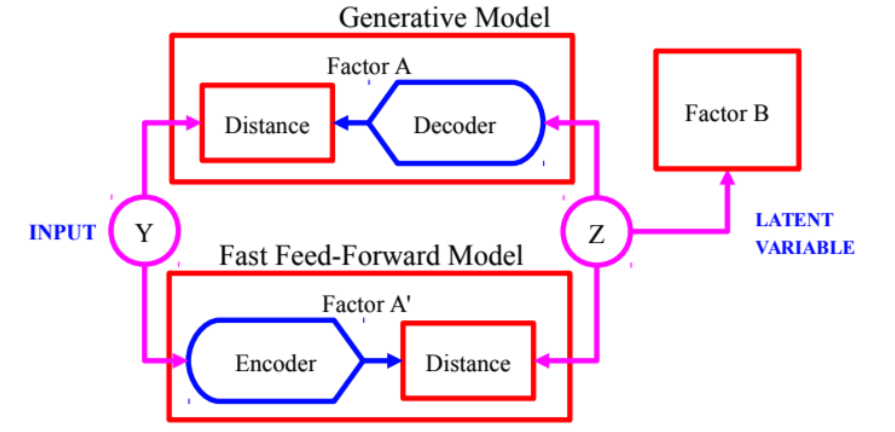
\includegraphics[scale=0.4]{lectures/12-a/enco_deco.png}
\caption{Encoder-Decoder Architecture}
\label{enco_deco}
\end{figure}

The reason why the information content of the code has to be reduced is because otherwise the learning is not successful. In fact, when trained by minimizing the reconstruction error over the training set without any additional component, the algorithm does not learn structure from training sample, but rather it copies the data. Reducing the number of available features forces the algorithm to understand the underlying structure, which is why we reduce dimensions or introduce sparsity. Fig. \ref{code2} and Fig. \ref{reduce} give a graphical representation of such mechanism.

\begin{figure}[h]
\centering
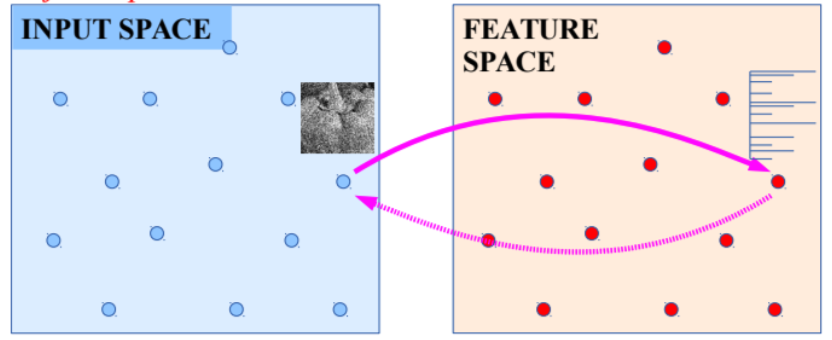
\includegraphics[width=1.0\linewidth]{lectures/12-a/code2.png}
\caption{Encoding without reducing the number of features}
\label{code2}
\end{figure}

\begin{figure}[h]
\centering
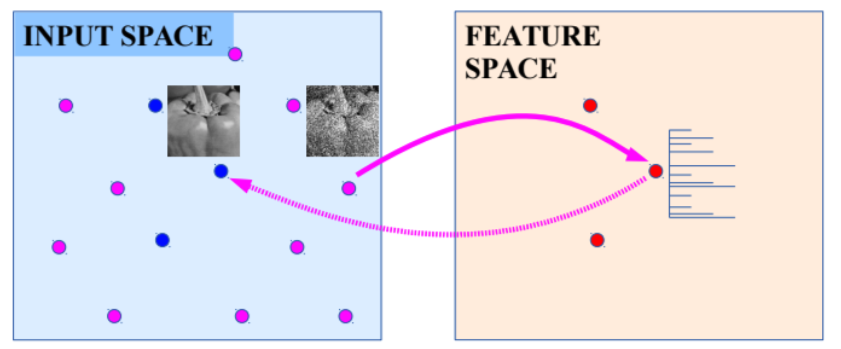
\includegraphics[width=1.0\linewidth]{lectures/12-a/reduce_code.png}
\caption{Encoding while reducing the number of available features.}
\label{reduce}
\end{figure}


\subsection{Predictive Sparse Decomposition (PSD): sparse auto-encoder}

Predictive Sparse Decomposition (PSD) \cite{kavukcuoglu2010fast}, illustrated in Fig \ref{Sparse AE} predicts the optimal code with a trained encoder. The mathematical formulation is the following:

\[\begin{array}{l}{E\left(Y^{i}, Z\right)=\left\|Y^{i}-W_{d} Z\right\|^{2}+\left\|Z-g_{e}\left(W_{e}, Y^{i}\right)\right\|^{2}+\lambda \sum_{j}\left|z_{j}\right|} \\ {g_{e}\left(W_{e}, Y^{i}\right)=S_{\lambda}\left(W_{e} Y^{i}\right)}\end{array}\]
where $S_{\lambda}$ is the shrinkage function, defined as
\[
S_{\lambda}(x)=\max\{|x|-\lambda,0\}\operatorname{sign}(x)
\]

\begin{figure}[h]
\centering
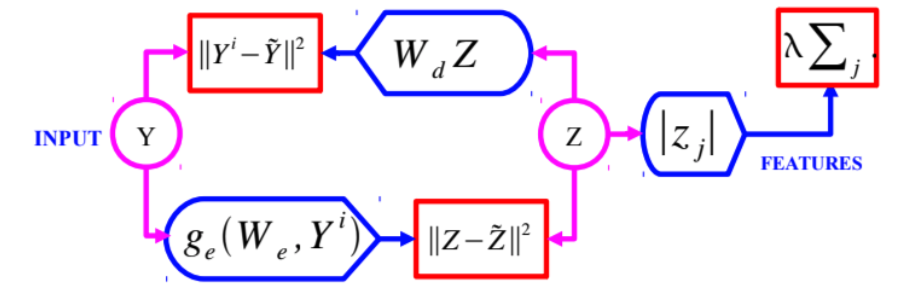
\includegraphics[scale=0.4]{lectures/12-a/PSD.png}
\caption{Sparse Autoencoder}
\label{Sparse AE}
\end{figure}

Fig \ref{basis} shows the basis functions (and encoder matrix) as digit parts when applying PSD to the MNIST dataset. Each patch here represents a columns of $W_d$. On the other hand, Fig \ref{natural_0} and Fig \ref{natural} shows training PSD on natural images. The patch of inputs being reconstructed is the combination of small group of edges called wavelets in the signal processing field.

\begin{figure}[H]
\centering
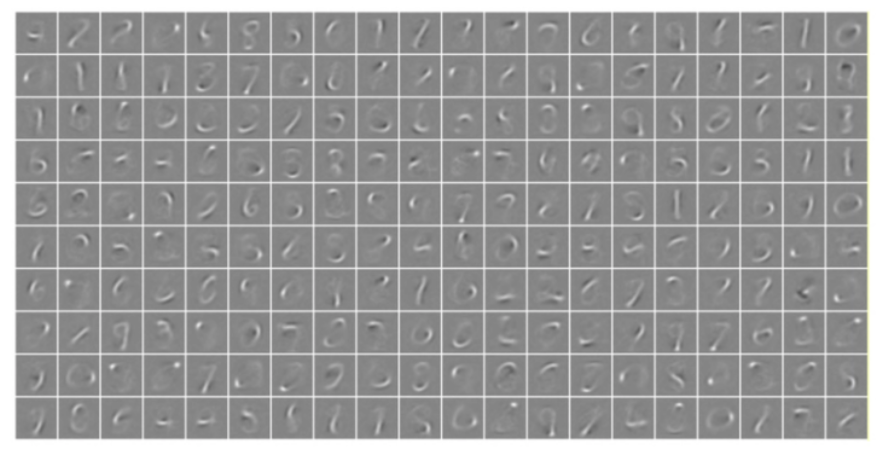
\includegraphics[scale=0.4]{lectures/12-a/basis.png}
\caption{PSD: Basis Functions on MNIST}
\label{basis}
\end{figure}

\begin{figure}[H]

\begin{minipage}[b]{.4\textwidth}
  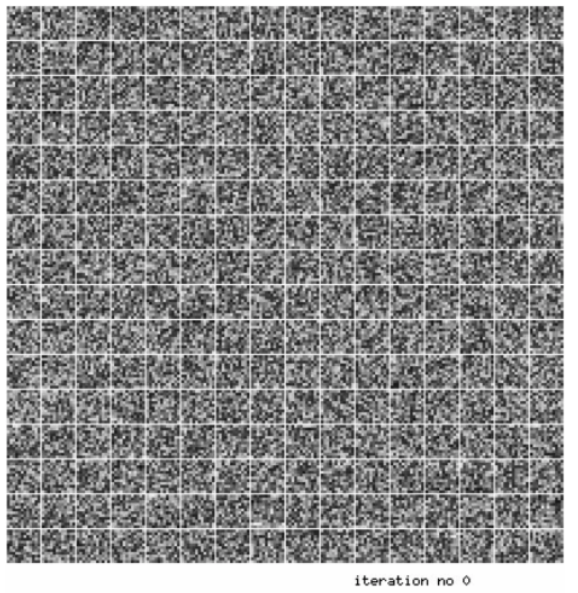
\includegraphics[width=\textwidth,left]{lectures/12-a/natural_0.png}
  \caption{Training on natural images patches}
  \label{natural_0}
\end{minipage}
\begin{minipage}[b]{.4\textwidth}
  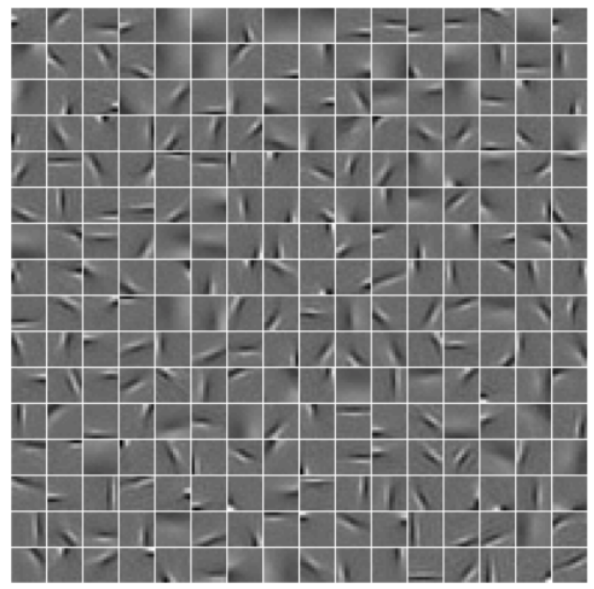
\includegraphics[width=\textwidth,right]{lectures/12-a/natural.png}
  \caption{Learned Features on natural patches:
V1-like receptive fields}
  \label{natural}
\end{minipage}
\end{figure}

%\begin{figure}[H]
%\centering
%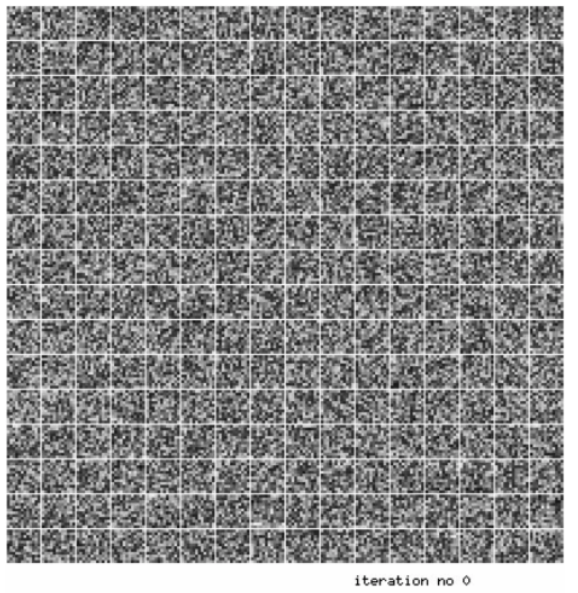
\includegraphics[width=1.0\linewidth]{lectures/12-a/natural_0.png}
%\caption{Training on natural images patches.}
%\label{natural_0}
%\end{figure}

%\begin{figure}[H]
%\centering
%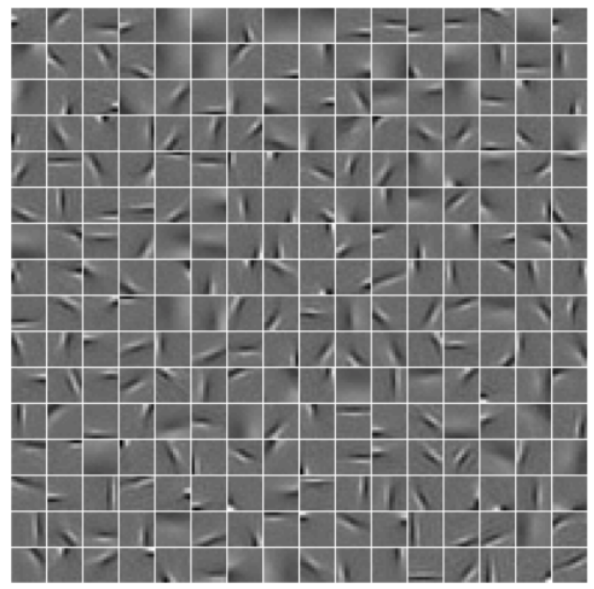
\includegraphics[width=1.0\linewidth]{lectures/12-a/natural.png}
%\caption{Learned Features on natural patches:
%V1-like receptive fields}
%\label{natural}
%\end{figure}

%end of Bingqian part, beginning of Ambuj
\section{Learning to infer LISTA}

LISTA is a method which has general application and is being increasingly used. It consists in training a neural network to solve optimization for an inverse problem in sparse coding. 
LISTA takes its name from the ISTA algorithm, a previously known method from sparse coding.
With a sparse auto encoder, a simple neural network is trained to predict what the encoder was. Firstly proposed by Gregor and LeCun in \cite{gregor2010learning}, it involves training a neural network to make the prediction in such a way that the output of this neural network allows to implement the ISTA algorithm, whose basic step is summarized below:

\[
Z(t+1) = S_{\frac{\lambda}{L}}[Z(t) - \frac{W_d ^ T (W_d Z(t) - Y)}{L}] 
\]
The ISTA algorithm takes the current value of the latent vector, subtracts the reconstruction error and subsequently applies a shrinkage by an amount $\frac{\lambda}{L}$, where $\lambda$ is the coefficient of the sparsity term. This equation looks very similar to a recurrent net with two sided values.

A RNN-based architecture as in Figure \ref{fig:fistaFlowGraph} is used to predict an optimal $Z$ and allows to limit the number of iterations through time.

An alternative mathematical form is given by
\[Z(t+1) = S_{\frac{\lambda}{L}}[W_e ^T Y + SZ(t)]\]

where
\[W_e = \frac{W_d}{L} \quad\quad S = I - \frac{ W_d ^T W_d}{L}\]

These are learned by running the recurrent net multiple times, in order to get as close as possible to the optimal solution that could be obtained by running stochastic conversion.


\begin{figure}[H]
  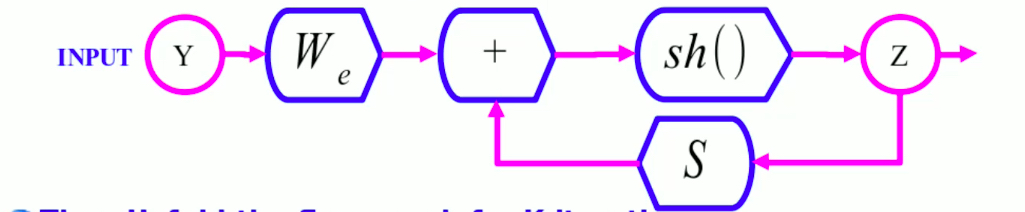
\includegraphics[width=\linewidth]{lectures/12-a/FISTAFlowGraph.jpg}
  \caption{LISTA flow graph}
  \label{fig:fistaFlowGraph}
\end{figure}

Fig.\ref{fig:fistaFlowGraph} shows the architecture of the neural network. At each temporal step our input Y is multiplicated by a matrix $W_e$ and added to a linear transformation of the output from the previous time step $Z(t)$. The new output is then obtained by passing the previous result through a non-linear shrinkage operation. The iterations proceed until a near-optimal solution is reached. Fig \ref{fig:fistaFlowGraphTimeUnfold} shows the time-unfolded structure: 

\begin{figure}[H]
  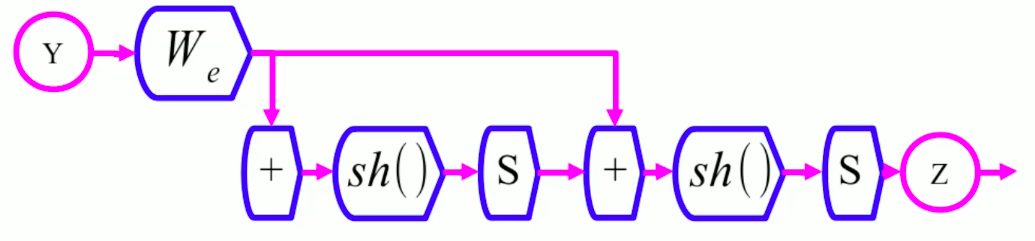
\includegraphics[width=\linewidth]{lectures/12-a/FISTAFlowGraphTimeUnfold.jpg}
  \caption{LISTA flow graph time unfold}
  \label{fig:fistaFlowGraphTimeUnfold}
\end{figure}

The matrices $W_e$ and $S$ are weights that can be learned with backpropagation-through-time within a fixed number of iterations $K$, serving as a hyperparameter.

Fig. \ref{fig:listaFista} shows the performance of LISTA in comparison with the fast version of ISTA (FISTA). The horizontal axis represents the number of iterations to produce the energy-minimizing $Z$, while the vertical axis represents the reconstruction error. 


\begin{figure}[h!]
  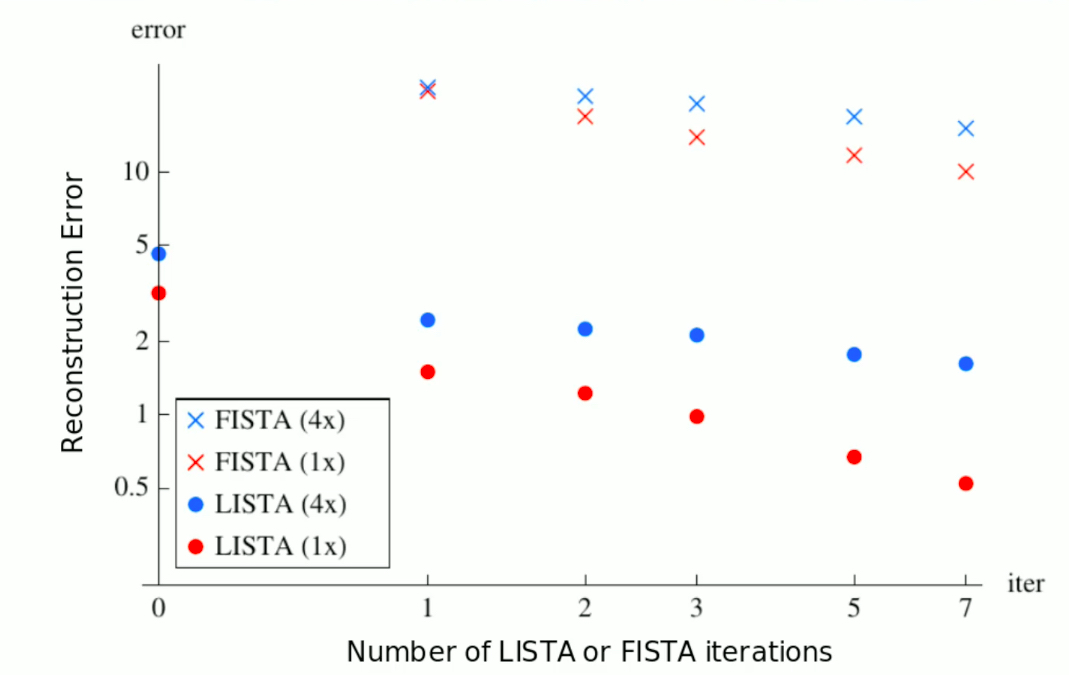
\includegraphics[width=\linewidth]{lectures/12-a/FISTALISTA.jpg}
  \caption{Learning ISTA Vs ISTA/FISTA}
  \label{fig:listaFista}
\end{figure}

The reconstruction error decreases much faster for LISTA, which is surprising, considering that we are comparing a neural network to an algorithm that actually optimizes the function. However, the reason for this discrepancy is that we are not solving a general problem, but rather we are training it to perform well on the available data. If tested on different data, the algorithm would not perform as well, which is the price to pay to get a speed improvement. 

\section{Convolutional Sparse Coding} 
In Convolutional Sparse Coding, the input $Y$ is a full image instead of a vector and each component $Z_k$ of the sparse code is a feature map (an image). The following equation represents the reconstruction error for regular Sparse Coding, with $L^1$ regularization:
\[E(Y,Z) = ||Y - \underset{k}{\Sigma} W_k Z_k||^2 + \alpha \underset{k}{\Sigma}|Z_k|\]
Notice that the energy function in this case is a scalar quantity. In Convolutional Sparse Coding, instead, the scalar code component $Z_k$ is replaced by a feature map and the multiplication is replaced by convolution. The structural problem therefore becomes that of reconstructing an image as a sum of feature maps, after convolution by vectors is applied. In order to do so, convolution filters are learned as if they were the encoder matrix $W_d$ of the previous problem

\[E(Y,Z) = ||Y - \underset{k}{\Sigma} W_k * Z_k||^2 + \alpha \underset{k}{\Sigma}|Z_k|\]

Fig.\ref{fig:PATCHvCONV} compares features that are learned through the two different methods when we train our system on patches of 12 by 12 pixel each.

In the case of patch-based learning, the system has learned to produce a shifted version of the filters to be able to reconstruct the image, as it needs to model separately every position, angle, scale and so on. However, in case of convolutional-based learning, the convolutional nature of the architecture filters all the possible shifts, so that the system doesn't need to have separate filters at every location within the window. This is why the training is devoted to learn more diverse filters as shown in the figure.

\begin{figure}[H]
  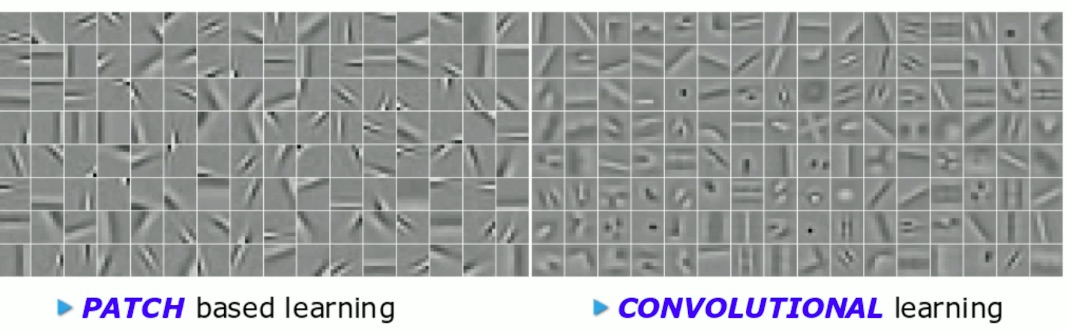
\includegraphics[width=\linewidth]{lectures/12-a/PATCHvCONV.jpg}
  \caption{Patch based Learning Vs Convolutional Learning}
  \label{fig:PATCHvCONV}
\end{figure}

Below (Fig.\ref{fig:MultipleFilters}) are the filters we get from a system which has an auto-encoder with a layer of non-linearity and a linear decoder. 
\begin{figure}[H]
  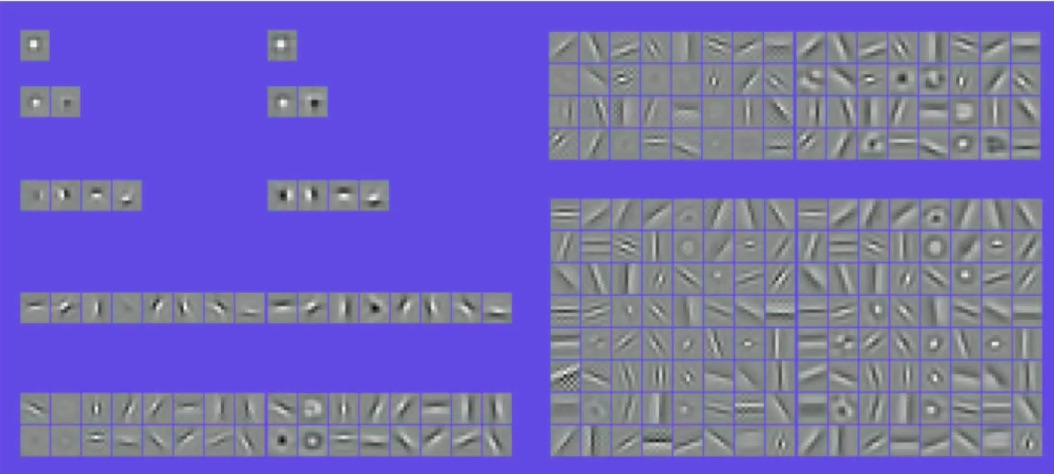
\includegraphics[width=\linewidth]{lectures/12-a/MultipleFilters.jpg}
  \caption{Filters and basis functions obtained with 1,2,4,8,16.32 and 64 filters}
  \label{fig:MultipleFilters}
\end{figure}
On the right side the components of $W_d$ and the encoder are shown, while on the left the decoder is represented (left and right are mirrors of each other). As the number of filters increases, there is more diversity in the type of filters. These filters are learned spontaneously by a convolutional neural network with unsupervised training on an a large image dataset. This suggests that are completely unsupervised ways of pre-training CNNs to learn features in fields where there is shortage of data, including magnetic imaging and speech translation.


\section{Using PSD to train a hierarchy of features}
PSD can also be used to train features on different layers. As a first step, the sparsity encoder is trained on raw data as a first layer using the aforementioned methods. Once a certain level of accuracy is reached, the iterations can be removed and the feature extractor can be considered, possibly with multiple layers in the encoder. These steps are visible in Fig. \ref{fig:0} and Fig. \ref{fig:1} 
\begin{figure}[h!]
  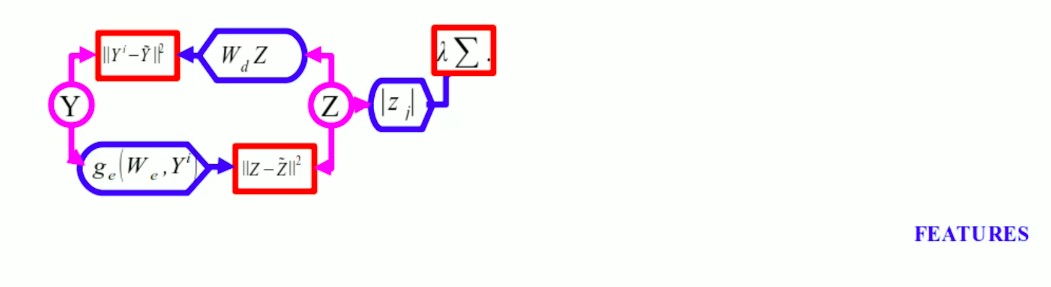
\includegraphics[width=\linewidth]{lectures/12-a/0.jpg}
  \caption{Step 1}
  \label{fig:0}
\end{figure}

\begin{figure}[h!]
  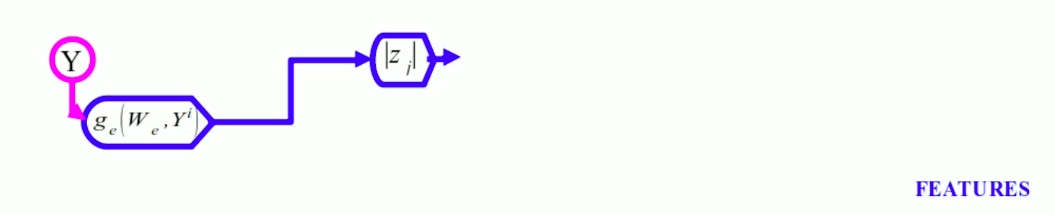
\includegraphics[width=\linewidth]{lectures/12-a/1.jpg}
  \caption{Step 2}
  \label{fig:1}
\end{figure}

Further, we generate data from the feature extractor and train a second layer using PSD. This will produce a second layer of feature extractor. These steps are visible in Fig. \ref{fig:2} and Fig. \ref{fig:3} 
\begin{figure}[h!]
  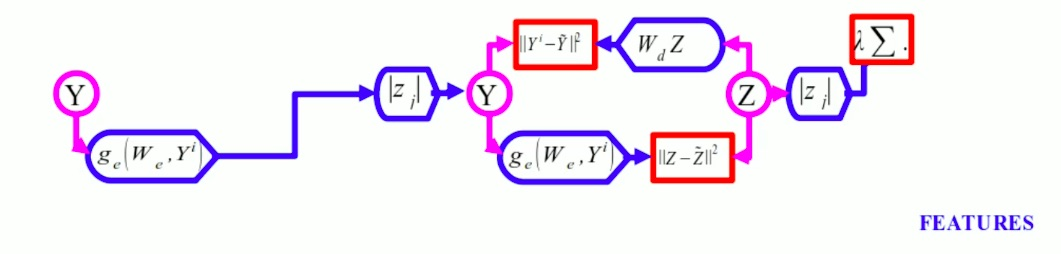
\includegraphics[width=\linewidth]{lectures/12-a/2.jpg}
  \caption{Step 3}
  \label{fig:2}
\end{figure}

\begin{figure}[h!]
  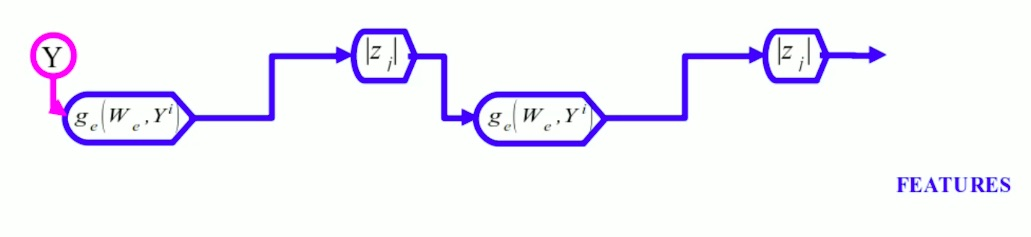
\includegraphics[width=\linewidth]{lectures/12-a/3.jpg}
  \caption{Step 4}
  \label{fig:3}
\end{figure}

There is now a two layers convolutional network that can extract features and has been trained through unsupervised learning. Possibilities for improvement include adding a supervised classifier as the top layer as in Fig.\ref{fig:4} or fine tune the entire system using supervised back-propagation.
\begin{figure}[h!]
  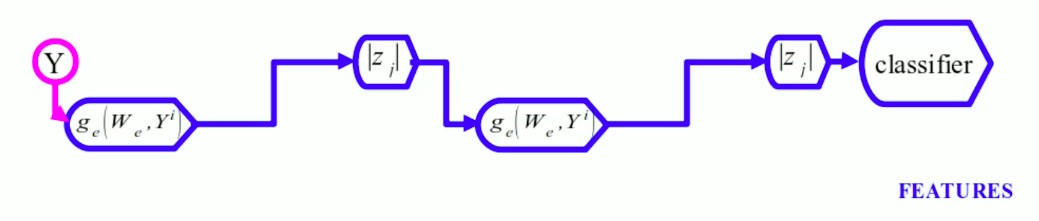
\includegraphics[width=\linewidth]{lectures/12-a/4.jpg}
  \caption{Step 5}
  \label{fig:4}
\end{figure}

\section{Sparse Auto-Encoder with Slow Feature Penalty}
One way to train a system to learn features is not to train on static images but rather train it on videos, exploiting the redundancy in videos for system to learn good features. For example, in order to learn live features, two successive frames of videos can be used. Moving objects forces the network to model two successive representation of inputs where the only modification comes from the position and the angle. Fig.\ref{fig:SlowPenalty} shows how the process works. 
\begin{figure}[H]
  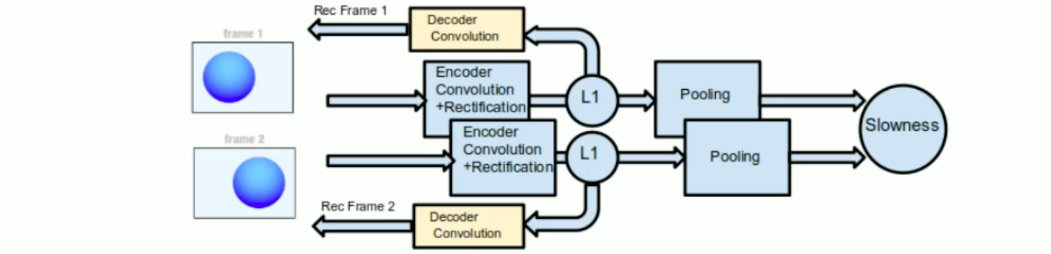
\includegraphics[width=\linewidth]{lectures/12-a/SlowPenalty.jpg}
  \caption{Sparse auto-encoder with 'slow feature' penalty}
  \label{fig:SlowPenalty}
\end{figure}


In particular, a frame is fed to an auto-encoder with $L^1$ regularization and then followed by a decoder layer. Then another frame is fed to the same auto-encoder. In this way it is possible to ensure that the information in the code contains enough data to properly reconstruct the input. After pooling over space and features, the algorithm is followed by a parameter objective function that ensures that both codes are identical (i.e. representations of the frames where objects have moved a little back should be identical). In other words, the algorithm needs to train filters which ensures that, after pooling, the frames are shifting back.

This method was originally called 'slow feature analysis' because it exploits the similarity of adjacent frames in a video to learn analogous embeddings by making sure the representation in successive frames is identical.


